\documentclass[a4paper,11pt]{article}
\usepackage[margin=2cm]{geometry}
\usepackage{graphicx}
\usepackage{float}
\usepackage{amsmath}
\usepackage{xcolor}
\usepackage{listings}
\usepackage{comment}
\usepackage{siunitx}


\lstdefinestyle{matlab}{
	language=Matlab,
	basicstyle=\ttfamily\footnotesize,
	keywordstyle=\color{blue!70!black},
	commentstyle=\color{green!40!black},
	stringstyle=\color{purple!80!black},
	numbers=left, numberstyle=\tiny\color{gray}, numbersep=6pt,
	frame=single, rulecolor=\color{gray!60},
	breaklines=true, breakatwhitespace=false,
	columns=fullflexible, keepspaces=true,
	showstringspaces=false, tabsize=4,
	captionpos=t, aboveskip=8pt, belowskip=8pt
}

\lstdefinestyle{ccode}{
	language=C,
	morekeywords={int16_t, int32_t, uint16_t, uint32_t, __interrupt, volatile},
	basicstyle=\ttfamily\footnotesize,
	keywordstyle=\color{blue!70!black},
	commentstyle=\color{green!40!black},
	stringstyle=\color{purple!80!black},
	directivestyle=\color{orange!70!black},
	numbers=left, numberstyle=\tiny\color{gray}, numbersep=6pt,
	frame=single, rulecolor=\color{gray!60},
	breaklines=true, breakatwhitespace=false,
	columns=fullflexible, keepspaces=true,
	showstringspaces=false, tabsize=4,
	captionpos=t, aboveskip=8pt, belowskip=8pt
}


\newcommand{\taskbox}[1]{%
	\noindent\fbox{\parbox{\dimexpr\linewidth-2\fboxsep-2\fboxrule}{#1\strut}}\par\medskip}

\title{ESP Lab2: Prep Sheet\\ \large Multirate FIR Branching Filter}

\begin{document}
	\sloppy
	\maketitle
	
	\begin{table}[h]
		\centering
		\begin{tabular}{|l|l|l|}
			\hline
			\textbf{Group / Team} & \textbf{Team member 1:} & Pham, Tuong Minh \\
			\hline
			ESPL/01 / & \textbf{Team member 2: } & Ul Haq, Waleed \\
			\hline
		\end{tabular}
	\end{table}
	
	\begin{table}[h]
		\centering
		\caption{Filter specifications of lab group ESPL/01}
		\small
		\begin{tabular}{|l|l|c|}
			\hline
			\textbf{Parameter} & & \textbf{ESPL/01} \\
			\hline
			Sampling rate of ADC and DAC & & $f_s = 50$\,kHz \\
			\hline
			Lowpass filter & passband edge & $f_{pass,LP} = 3100$\,Hz \\
			& stopband edge & $f_{stop,LP} = 3350$\,Hz \\
			\hline
			Complementary highpass filter & stopband edge & $f_{stop,HP} = 3100$\,Hz \\
			& passband edge & $f_{pass,HP} = 3350$\,Hz \\
			\hline
			Total passband ripple & & $\delta_{pass} = 0.01$ (linear, not dB) \\
			\hline
			Minimum stopband attenuation & & $\delta_{stop} = 40$\,dB \\
			\hline
			Quantisation of signals and coefficients & & 16 bit (1Q15 format) \\
			\hline
		\end{tabular}
	\end{table}
	
	\setcounter{section}{2}
	\section{Preparation}
	
	\subsection*{Use of generative AI}
	
	Tool: Claude (Anthropic). The lab instructions and the Moodle files were provided as context. Essential prompts (translated from German, condensed):
	\begin{enumerate}
		\item ``Create an empty LaTeX document for the preparation sheet of ESP Lab 2.''
		\item ``Section 3.1: Explain to me how the filter order of the single-rate solution is obtained from the MATLAB output of \texttt{dec\_kernel\_int\_WS20\_EMIL.m}, how many DSP cycles are available per sampling period and whether a real-time implementation is feasible.''
		\item ``Section 3.2: Explain to me how $M_{opt}$ is obtained with \texttt{roots\_demo.m} and how the edge frequencies and passband ripples of the decimation, interpolation and kernel filter are determined. Extend \texttt{dec\_kernel\_int\_WS20\_EMIL.m} as simply as possible with the filter design using \texttt{firpmord()}/\texttt{firpm()}, the magnitude plots and the export of the polyphase coefficients.''
		\item ``Explain to me why the cascade plot in MATLAB shows a higher stopband attenuation than a measured magnitude response of a multirate filter.''
		\item ``Section 3.3: Explain to me how the computational effort and the group delay of the single-rate and the multirate filter are calculated using the formulas from the lecture, and write the results as LaTeX text for the prep sheet.''
	\end{enumerate}
	

	\subsection{Conventional lowpass filter}
	
	\taskbox{Design a linear-phase FIR low-pass and its complementary high-pass using firpmord() and
		firpm(). Use the specification above und the script dec\_kernel\_int.m provided in Moodle. Plot both magnitude responses in dB for both filters in two different subplots. Verify $\delta_{pass}$
		and $\delta_{stop}$.}
	
	\begin{figure}[H]
		\centering
		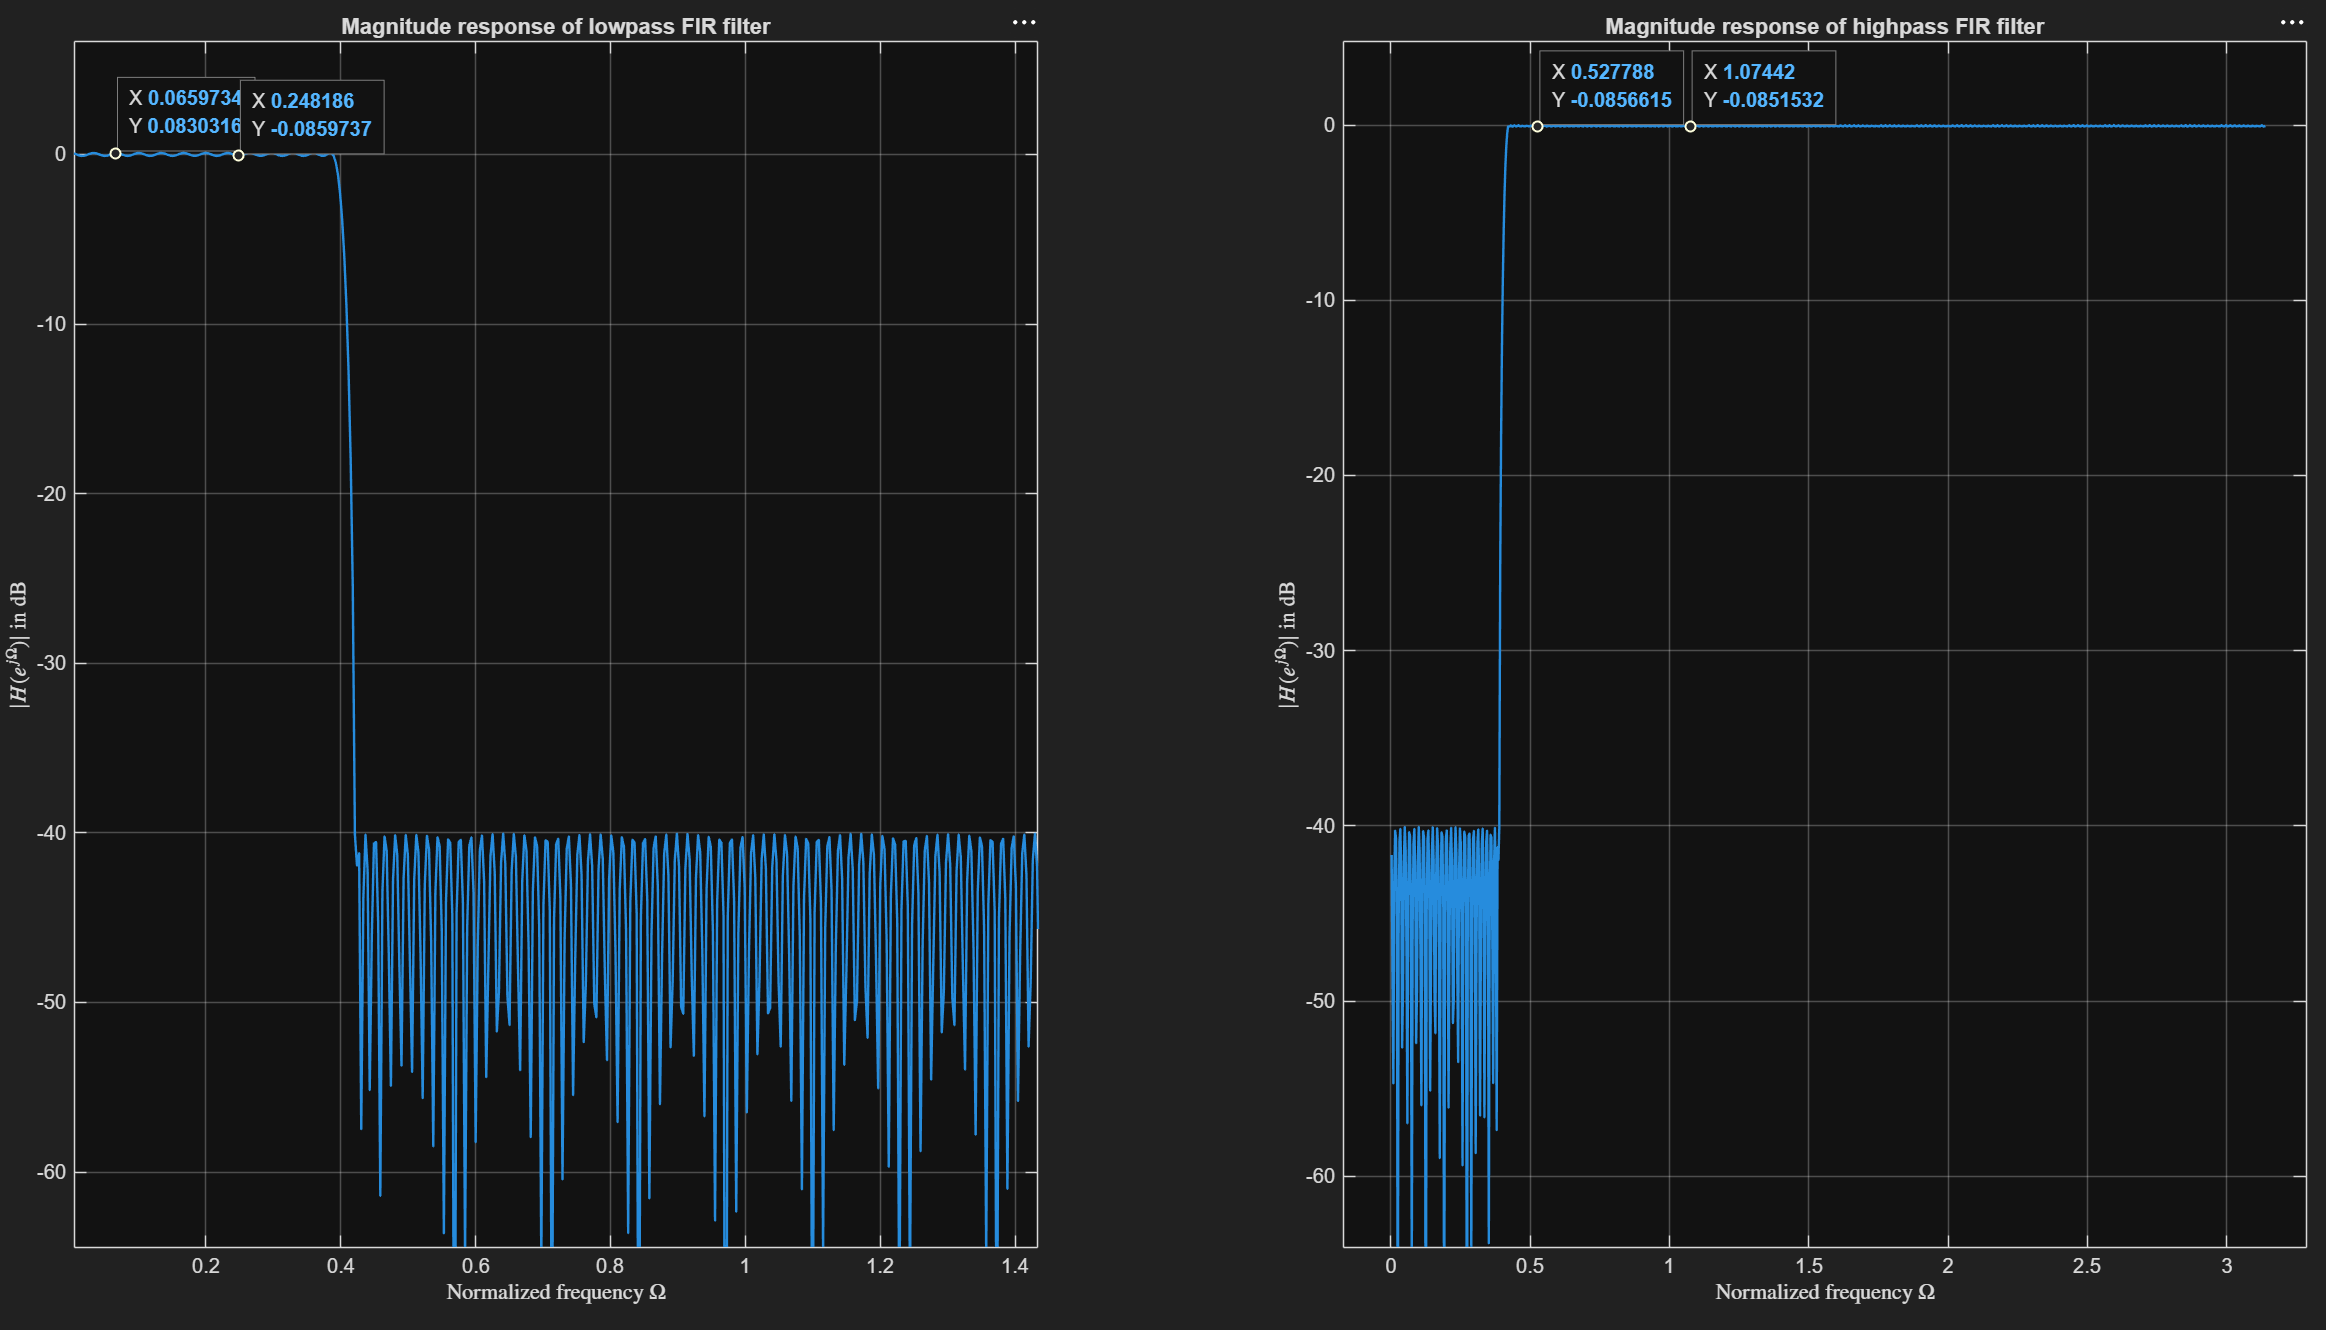
\includegraphics[width=1\linewidth]{3.1_normalfilter}
		\caption{Magnitude responses of the single-rate FIR low-pass (left) and the complementary high-pass (right), designed with \texttt{dec\_kernel\_int\_WS20\_EMIL.m}, $N = 391$.}
		\label{fig:3.1}
	\end{figure}
	
	\noindent\textbf{Verification.} Fig.~\ref{fig:3.1} shows a stopband attenuation of at least 40\,dB for both filters, so $\delta_{stop}$ is met. The maximum passband deviation read from the plot is about $\pm 0.085$\,dB. Converted to a linear value:
	\[
	10^{0.085/20} \approx 1.0098, \qquad 10^{-0.085/20} \approx 0.9902 \quad\Rightarrow\quad \left|\,|H| - 1\,\right| \approx 0.0098 \le \delta_{pass} = 0.01.
	\]
	The passband ripple therefore also meets the requirement. For comparison, $\delta_{pass} = 0.01$ corresponds to $20\log_{10}(1.01) \approx 0.086$\,dB.
	
	\taskbox{From the Matlab output, record the filter degree (order) for the single-rate solution.}
	
	\noindent\textbf{Filter order.} \texttt{firpmord()} estimates an order of 389; the script adds 2 as a safety margin, so the single-rate filter has the order $N = 391$ (MATLAB output: \texttt{N\_FIR=391}). An FIR filter of order $N$ computes $y[n] = \sum_{k=0}^{N} b_k\,x[n-k]$, so it has $N + 1 = 392$ coefficients. The high order is caused by the narrow transition band of only 250\,Hz compared to the sampling frequency ($\Delta f / f_s = 0.005$).
	
	\taskbox{Compute the DSP cycles available per sampling period at $f_s= 50\si{\kilo\hertz}$ and $f_{DSP}= 456\si{\mega\hertz}$.
		Discuss the feasibility of real-time implementation on the DSP without further code
		optimization.}
	
	\noindent At $f_{DSP} = 456$\,MHz and $f_s = 50$\,kHz, the number of DSP cycles available per sampling period is
	\[
	\frac{f_{DSP}}{f_s} = \frac{456\,\text{MHz}}{50\,\text{kHz}} = 9120 \text{ cycles}.
	\]
	The single-rate filter has 392 coefficients, i.e.\ 392 multiply-accumulate operations per sample plus the update of the delay line. With the optimised assembly routine \texttt{FIR\_filter\_asm\_sc.asm} ($16 + 6N$ cycles), the filter requires about $16 + 6 \cdot 392 \approx 2370$ cycles, i.e.\ about 26\,\% of the available time, so a real-time implementation is feasible. Without code optimisation (plain C), several cycles are needed per coefficient for loading, multiplying, accumulating and shifting the delay line. With an estimated 15 to 25 cycles per coefficient, the filter would take about 65\,\% to more than 100\,\% of the available cycles, which is at the limit of real-time operation. This high effort, caused by the narrow transition band, motivates the multirate implementation in Section 3.2.
	
	% ------------------------------------------------------------------
	\subsection{Multi-rate FIR filter design}
	\subsubsection{Optimum choice of downsampling/upsampling factor M}
	
	\taskbox{Add the exact value for $M_{opt}$ and the nearest integer number to the prep sheet.}
	
	\begin{lstlisting}[style=matlab, caption={\texttt{roots\_demo.m} with the specification of ESPL/01, Section 3.2.1}, label={lst:roots}]
		% roots_demo.m
		%
		% US 07-Nov-23
		%
		% demo for finding M_opt
		clear
		close all
		Fs = 50000;
		fpass = 3100;
		fstop = 3350;
		
		a = fstop^2 - fpass^2;
		b = -(fpass + fstop)^2;
		c = 2 * Fs  * (fpass   + fstop);
		d = -Fs^2;
		
		my_polynom = [a b c d]
		roots(my_polynom)
	\end{lstlisting}
	
	\begin{lstlisting}[style=matlab, numbers=none, caption={MATLAB command window output, Section 3.2.1}, label={lst:rootsout}]
		my_polynom =
		
		1.0e+09 *
		
		0.0016   -0.0416    0.6450   -2.5000
		
		ans =
		
		10.2352 +13.6434i
		10.2352 -13.6434i
		5.3296 + 0.0000i
	\end{lstlisting}
	
	\noindent\textbf{Result.} The cubic polynomial has one real root and a pair of complex conjugate roots. Only the real root is a valid down-/upsampling factor, so the optimum factor is
	\[
	M_{opt} = 5.3296 \approx 5 \quad \text{(nearest integer)}.
	\]
	For the lab tasks, $M = L = 4$ is used as specified in Table~2 of the assignment.
	
	\subsubsection{Decomposition into decimation, interpolation and kernel filter}
	
	\taskbox{Determine the passband and stopband edge frequencies of the decimation and the kernel filter and the passband ripple of both filters. Extend \texttt{dec\_kernel\_int.m} with the design of the FIR filters via \texttt{firpmord()} and \texttt{firpm()}, plot the magnitude responses of the decimation filter, the kernel filter and the cascade of all three filters, and write the coefficient sets to the header file. Explain the approach and the verification of the results.}
	
	\noindent\textbf{Filter parameters.} With $M = L = 4$, the low sampling frequency is $f_s' = f_s/M = 12.5$\,kHz. The kernel filter runs at $f_s'$ and realises the steep transition of the original low-pass filter. The decimation and interpolation filters run at $f_s$ and are identical.
	
	\begin{table}[H]
		\centering
		\caption{Theoretical filter parameters for $M = L = 4$}
		\footnotesize
		\begin{tabular}{|l|c|c|c|c|c|}
			\hline
			\textbf{Filter} & \textbf{Sampling rate} & $\boldsymbol{f_{pass}}$ & $\boldsymbol{f_{stop}}$ & $\boldsymbol{\delta_{pass}}$ & \textbf{Stopband att.} \\
			\hline
			Decimation / interpolation & $f_s = 50$\,kHz & 3100\,Hz & $f_s' - f_{stop,LP} = 9150$\,Hz & $0.01/3$ & 40\,dB \\
			Kernel & $f_s' = 12.5$\,kHz & 3100\,Hz & 3350\,Hz & $0.01/3$ & 40\,dB \\
			\hline
		\end{tabular}
	\end{table}
	
	\noindent The kernel filter keeps the passband and stopband edges of the original filter, $f_{pass} = 3100$\,Hz and $f_{stop} = 3350$\,Hz.
	
	The decimation filter has the same passband edge of 3100\,Hz, so that the wanted signal passes unchanged. Its stopband edge only has to prevent aliasing into the range below $f_{stop,LP}$: after downsampling, a component at $f$ appears at $f_s' - f$. All components between $f_{stop,LP}$ and $f_s' - f_{stop,LP}$ are therefore folded into the stopband of the kernel filter and are removed there. Only components above $f_s' - f_{stop,LP} = 12.5\,\text{kHz} - 3.35\,\text{kHz} = 9.15$\,kHz would fall below $f_{stop,LP}$ and must be suppressed by the decimation filter. The same holds for the interpolation filter: the images of the kernel output (0 to 3350\,Hz) start at $f_s' - f_{stop,LP} = 9.15$\,kHz. This wide transition band (3100\,Hz to 9150\,Hz) allows a short decimation and interpolation filter.
	
	The signal passes through three filters in cascade (decimation, kernel and interpolation filter). In the worst case, their passband ripples add up. Each filter is therefore designed with one third of the total ripple, $\delta_{pass} = 0.01/3 \approx 0.0033$. The minimum stopband attenuation of 40\,dB is kept for each filter.
	
	\noindent\textbf{MATLAB implementation.} Listing~\ref{lst:m322} shows the code added to \texttt{dec\_kernel\_int\_WS20\_EMIL.m}. Both filters are designed with \texttt{firpmord()} and \texttt{firpm()}, including the safety margin of 2 as for the single-rate filter. The MATLAB output is \texttt{N\_FIR\_Dec\_Int = 20} and \texttt{N\_FIR\_kernel = 116}. The decimation filter is split into $M = 4$ polyphase filters with the coefficients $b_{Dec}[kM + \lambda]$, $\lambda = 0, \dots, 3$; the interpolation filter uses the same coefficient sets with its own delay lines. All coefficient sets are written to \texttt{dec\_kernel\_int\_WS20\_EMIL.h} with \texttt{write\_coeff.m}.
	
	\begin{lstlisting}[style=matlab, caption={Design of the decimation/interpolation and kernel filter, magnitude plots and header export, added to \texttt{dec\_kernel\_int\_WS20\_EMIL.m}, Section 3.2.2}, label={lst:m322}]
		% ---- 3.2 multirate filter design ----
		% optimum factor (see roots_demo.m) and factor for the lab (Table 2)
		r = roots([fstop^2-fpass^2, -(fpass+fstop)^2, 2*Fs*(fpass+fstop), -Fs^2]);
		MMmin = real(r(abs(imag(r)) < 1e-6));
		MM = 4;
		Fs_low = Fs/MM;
		
		% decimation / interpolation filter (at Fs), ripple 1/3 each
		fpass_dec = fpass;                % 3100 Hz
		fstop_dec = Fs_low - fstop;       % 12500 - 3350 = 9150 Hz
		[N_FIR_Dec_Int,fo,mo,w] = firpmord([fpass_dec fstop_dec], [1 0], [delta_pass/3 delta_stop], Fs);
		N_FIR_Dec_Int = N_FIR_Dec_Int + 2;
		b_dec = firpm(N_FIR_Dec_Int,fo,mo,w);
		
		% kernel filter (at Fs/M), ripple 1/3
		[N_FIR_kernel_MM,fo,mo,w] = firpmord([fpass fstop], [1 0], [delta_pass/3 delta_stop], Fs_low);
		N_FIR_kernel_MM = N_FIR_kernel_MM + 2;
		b_kernel = firpm(N_FIR_kernel_MM,fo,mo,w);
		
		fprintf('\n M_opt = %.4f, M = %d, N_FIR_Dec_Int = %d, N_FIR_kernel = %d\n\n', ...
		MMmin, MM, N_FIR_Dec_Int, N_FIR_kernel_MM);
		
		% magnitude responses at Fs
		f = linspace(0, Fs/2, 4000);
		H_dec = freqz(b_dec, 1, f, Fs);
		H_ker = freqz(b_kernel, 1, f, Fs_low);   % kernel runs at Fs/M -> periodic with Fs/M
		
		figure;                                  % decimation and kernel filter in one plot
		plot(f/1e3, db(H_dec)), hold on
		plot(f/1e3, db(H_ker)), grid
		axis([0 Fs/2e3 -80 5]);
		legend('Decimation / interpolation filter', 'Kernel filter (at f_s/M, periodic)');
		title('Magnitude response (dB)'); xlabel('f in kHz'); ylabel('|H| in dB');
		
		figure;                                  % cascade of the three filters
		plot(f/1e3, db(H_dec.*H_ker.*H_dec)), grid
		title('Cascade: decimation, kernel, interpolation filter'); xlabel('f in kHz');
		
		% ---- header file (inserted before the last fclose) ----
		% polyphase filters of the decimation filter (also used for interpolation)
		N_poly = ceil(length(b_dec)/MM);
		fprintf(file_ID, '#define N_delays_poly %d\n\n', N_poly);
		for lambda = 0:MM-1
		fprintf(file_ID, 'short H_dec_%d_delays[N_delays_poly];\n', lambda);
		fprintf(file_ID, 'short H_int_%d_delays[N_delays_poly];\n', lambda);
		write_coeff(file_ID, sprintf('b_poly_%d', lambda), b_dec(lambda+1:MM:end), N_poly);
		end
		
		% kernel filter
		fprintf(file_ID, '#define N_delays_kernel %d\n', length(b_kernel));
		fprintf(file_ID, 'short H_kernel_delays[N_delays_kernel];\n');
		write_coeff(file_ID, 'b_kernel', b_kernel, length(b_kernel));
	\end{lstlisting}
	
	\begin{figure}[H]
		\centering
		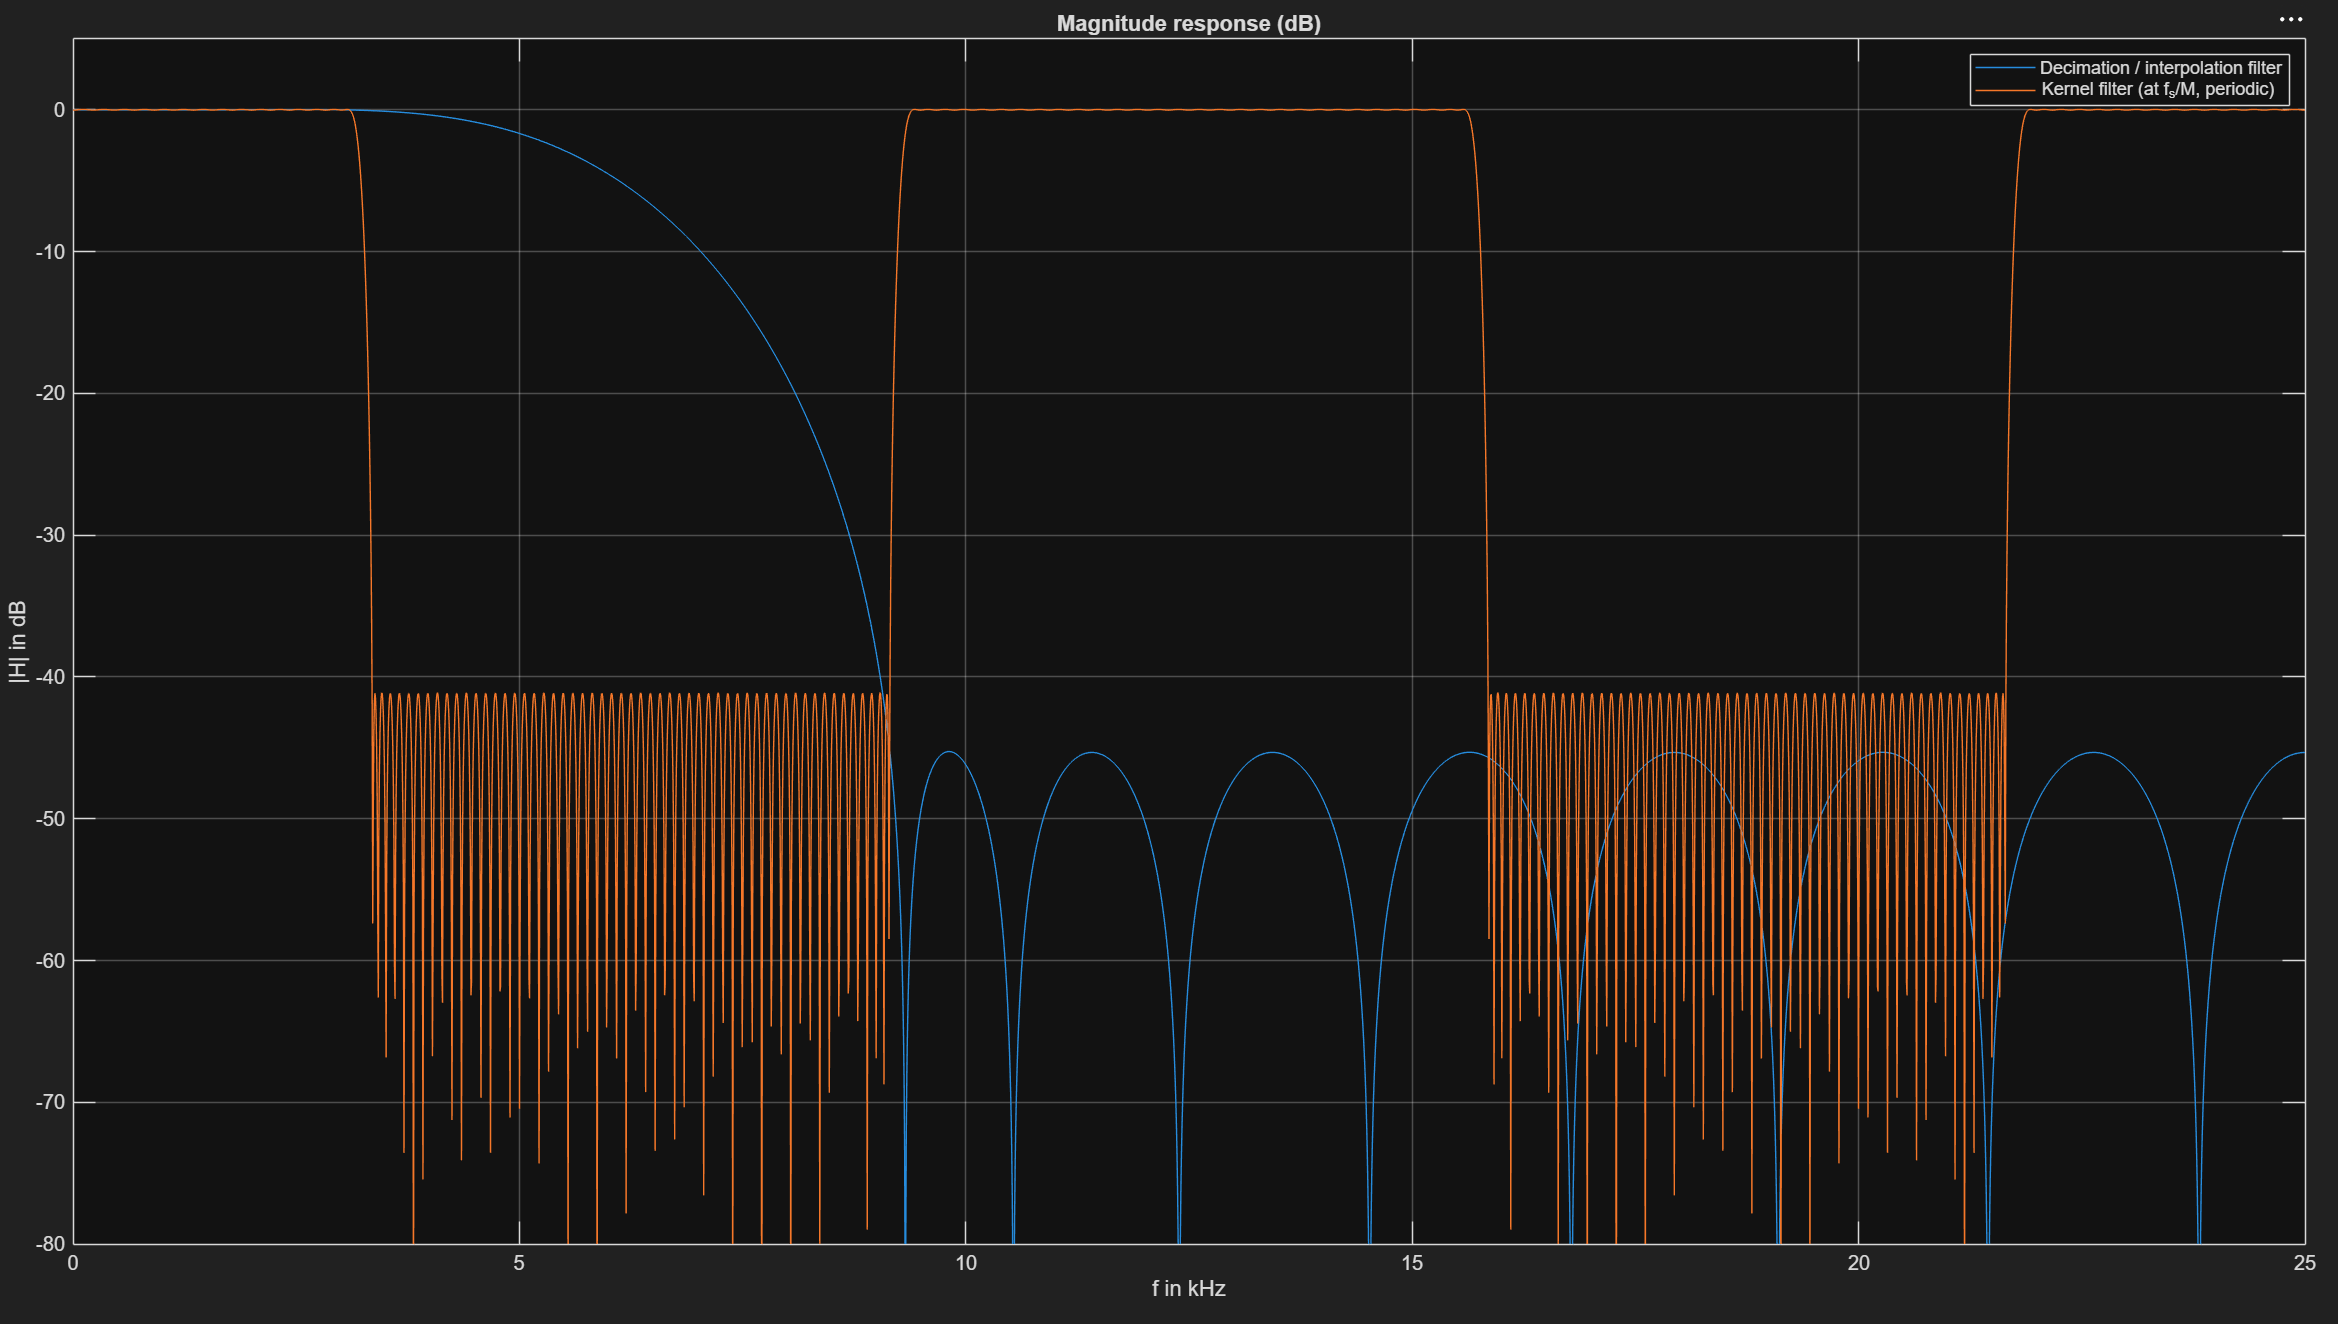
\includegraphics[width=1\linewidth]{3.2.3_kernel_int_dec}
		\caption{Magnitude responses of the decimation/interpolation filter (at $f_s$) and of the kernel filter (at $f_s/M$, periodic with $f_s' = 12.5$\,kHz).}
		\label{fig:322overlay}
	\end{figure}
	
	\begin{figure}[H]
		\centering
		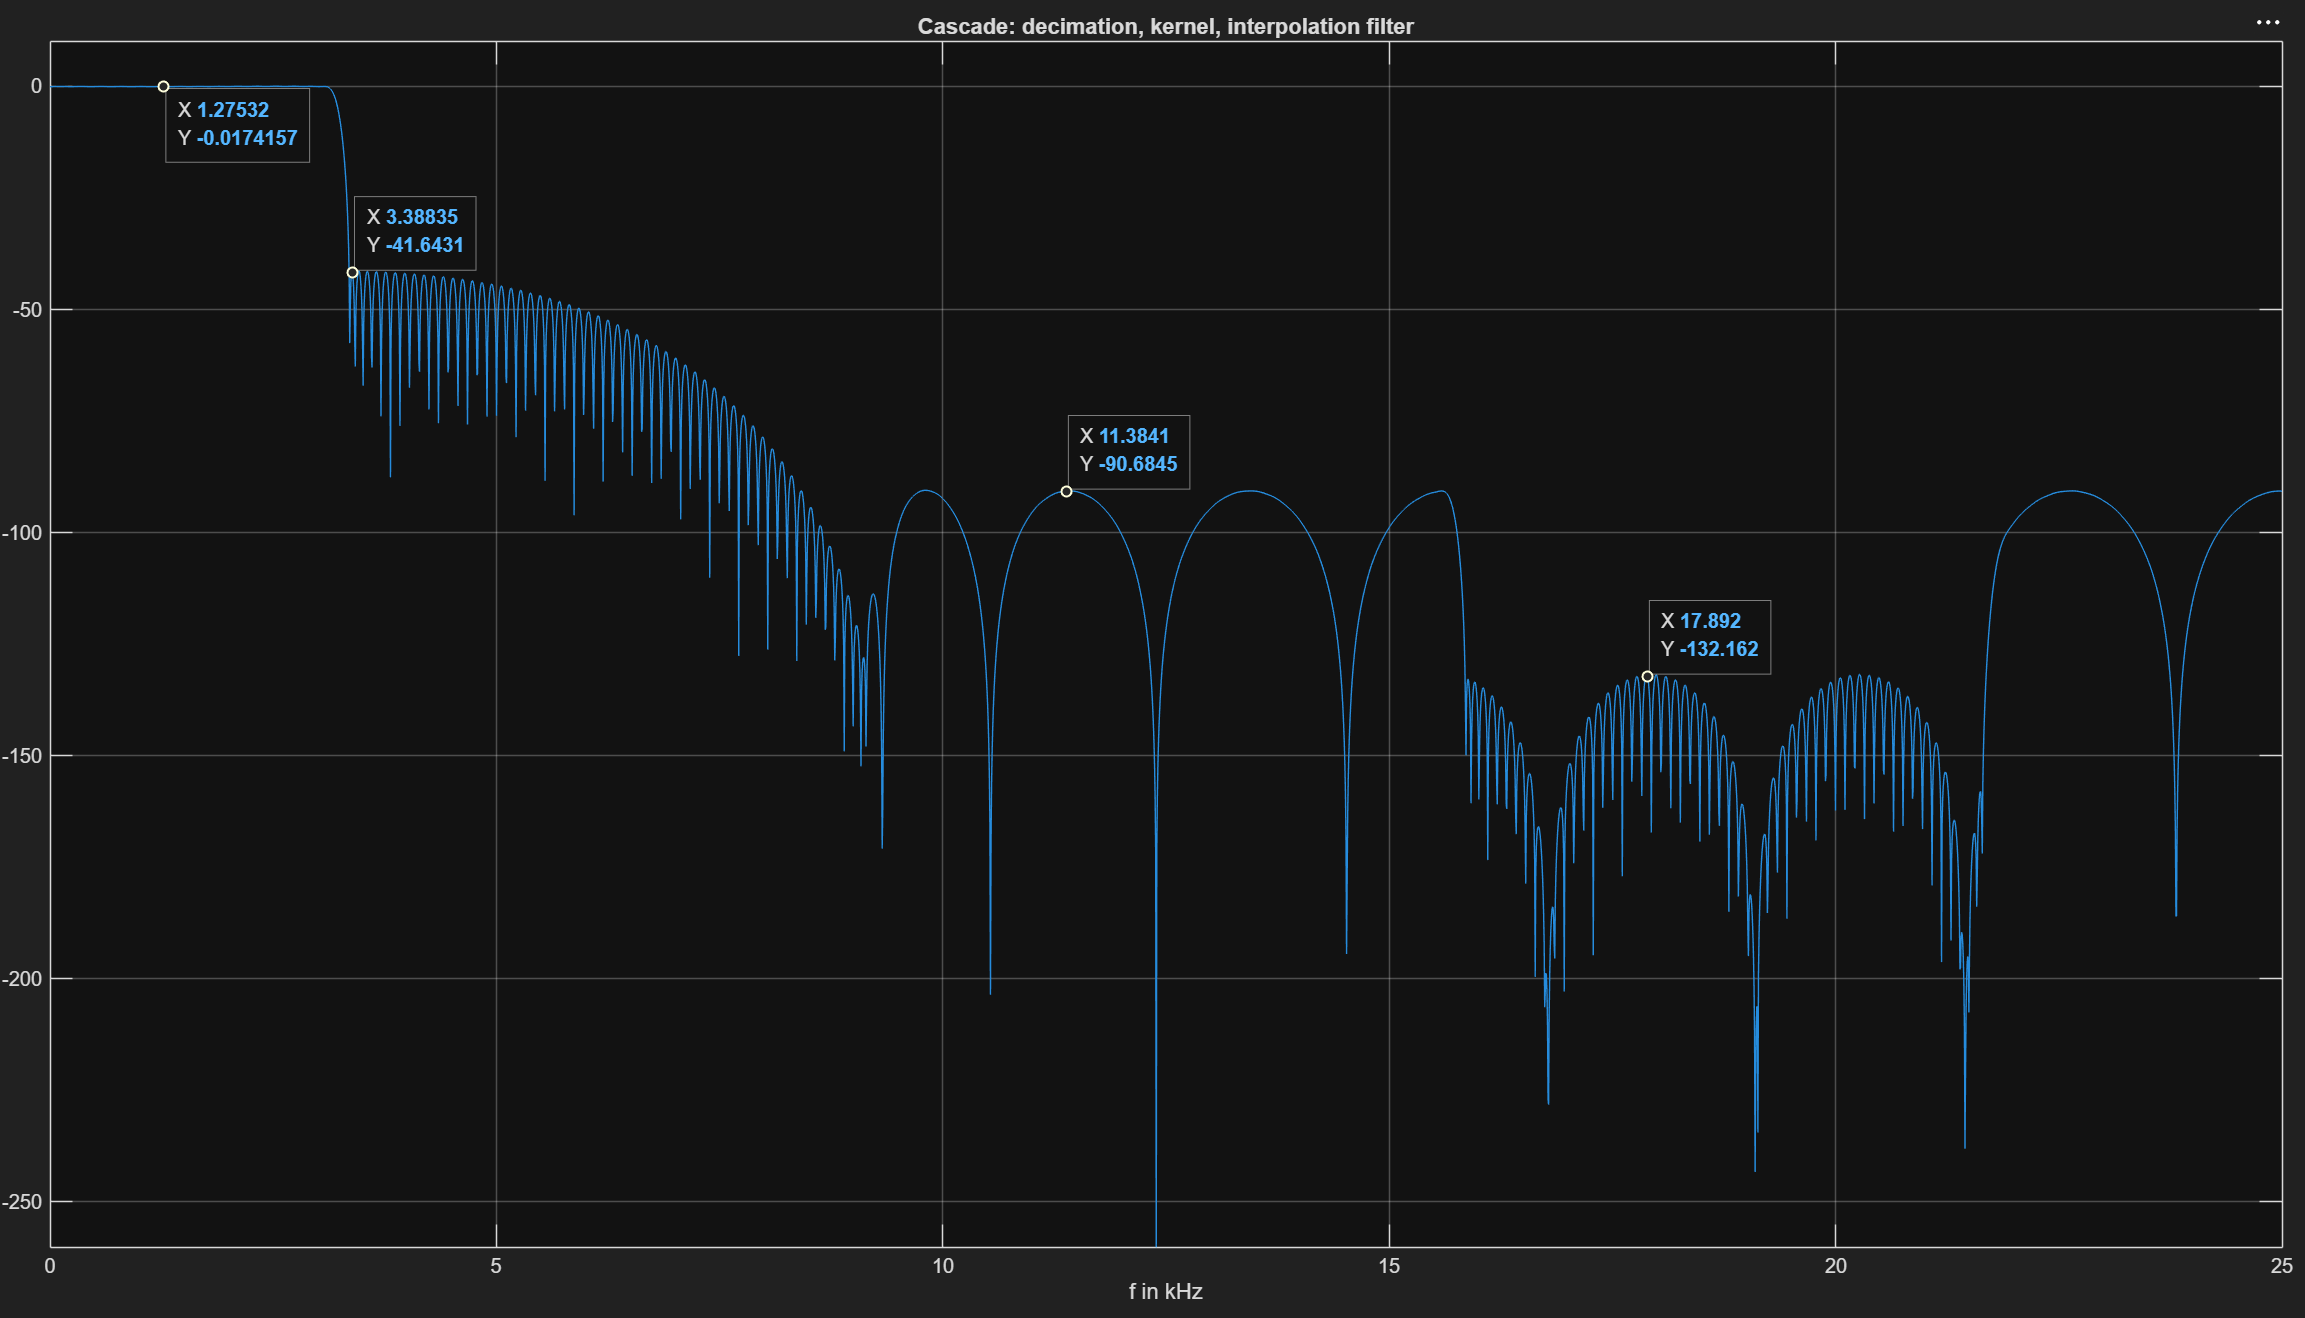
\includegraphics[width=1\linewidth]{3.2.3_}
		\caption{Magnitude response of the cascade of decimation, kernel and interpolation filter.}
		\label{fig:322cascade}
	\end{figure}
	
	\noindent\textbf{Verification.} Fig.~\ref{fig:322overlay} acts as a sketch of the spectra. Because the kernel filter runs at $f_s' = 12.5$\,kHz, its passband repeats at multiples of $f_s'$, i.e.\ at 9.4 to 15.6\,kHz and above 21.9\,kHz. All of these repetitions lie in the stopband of the decimation/interpolation filter, which starts at 9.15\,kHz. The decimation filter therefore prevents aliasing into the kernel passband, and the interpolation filter removes the corresponding images. In the frequency range between 3.35\,kHz and 9.15\,kHz, the decimation filter does not attenuate, but here the kernel filter provides at least 40\,dB.
	
	The cascade in Fig.~\ref{fig:322cascade} meets the specification: the passband deviation is below 0.02\,dB and the stopband attenuation is at least 41.6\,dB (at 3.39\,kHz). Note that this cascade response $H_{Dec}(f)\,H_{Kernel}(f)\,H_{Int}(f)$ neglects aliasing: input components near multiples of $f_s'$ are folded into the passband by downsampling and are then only attenuated once by the stopband of the decimation filter. In a measurement, the attenuation in these regions is therefore about 45\,dB instead of about 90\,dB shown in the plot, which still meets the specification.
	
	
	
	
	\begin{lstlisting}[style=ccode, caption={Generated header file \texttt{dec\_kernel\_int\_WS20\_EMIL.h} with the polyphase coefficients of the decimation/interpolation filter and the kernel coefficients, Section 3.2.2}, label={lst:header322}]
		//-------------------------------------------
		// designed with -- dec_kernel_int_WS20_EMIL.m --
		// Fs = 50000.00
		// MMmin =   5.33
		// fstop = 3350.00
		// fpass = 3100.00
		// delta_pass =   0.01
		// delta_stop_dB =  40.00
		// N_FIR = 391, instead two stages with N_FIR_Dec_Int = 20, N_FIR_KERNEL = 116
		//-------------------------------------------
		#define N_delays_poly 6
		short H_dec_0_delays[N_delays_poly];
		short H_int_0_delays[N_delays_poly];
		short b_poly_0[6]={
			218,  -1026,   4930,   4930,  -1026,    218,
		};
		short H_dec_1_delays[N_delays_poly];
		short H_int_1_delays[N_delays_poly];
		short b_poly_1[6]={
			248,  -1086,   7339,   2101,   -462,      0,
		};
		short H_dec_2_delays[N_delays_poly];
		short H_int_2_delays[N_delays_poly];
		short b_poly_2[6]={
			51,    -87,   8286,    -87,     51,      0,
		};
		short H_dec_3_delays[N_delays_poly];
		short H_int_3_delays[N_delays_poly];
		short b_poly_3[6]={
			-462,   2101,   7339,  -1086,    248,      0,
		};
		#define N_delays_kernel 117
		short H_kernel_delays[N_delays_kernel];
		short b_kernel[117]={
			63,   -104,     -1,     39,    -15,    -55,
			12,     56,    -23,    -64,     32,     69,
			-46,    -74,     62,     77,    -80,    -78,
			101,     77,   -124,    -72,    149,     63,
			-176,    -50,    205,     32,   -235,     -8,
			267,    -22,   -298,     61,    330,   -108,
			-362,    166,    394,   -236,   -424,    323,
			452,   -430,   -478,    565,    502,   -742,
			-523,    986,    541,  -1354,   -555,   1987,
			565,  -3417,   -571,  10410,  16957,  10410,
			-571,  -3417,    565,   1987,   -555,  -1354,
			541,    986,   -523,   -742,    502,    565,
			-478,   -430,    452,    323,   -424,   -236,
			394,    166,   -362,   -108,    330,     61,
			-298,    -22,    267,     -8,   -235,     32,
			205,    -50,   -176,     63,    149,    -72,
			-124,     77,    101,    -78,    -80,     77,
			62,    -74,    -46,     69,     32,    -64,
			-23,     56,     12,    -55,    -15,     39,
			-1,   -104,     63,};
	\end{lstlisting}
	
	
	
	
	
	
	
	
	
	% ------------------------------------------------------------------
	\subsection{Comparison of computational effort}
	
	\taskbox{Compare the computational effort $E_{total,single}$ of the original filter and $E_{total,multi}$ of the multirate filter for $M = L = 4$: order of the decimation/interpolation filter, order of the kernel filter, computational effort. How probable is a successful real-time implementation? Determine the group delay $\tau$ of the conventional and the multirate filter.}
	
	\noindent\textbf{Filter orders.} From the MATLAB output: decimation / interpolation filter $N_{Dec,Int} = 20$, kernel filter $N_{Kernel} = 116$ (both including the safety margin of 2), compared to $N = 391$ for the single-rate filter. The approximation from the lecture, $N_{FIR} \approx \frac{2}{3}\log_{10}\!\left(\frac{3}{10\,\delta_{pass}\delta_{stop}}\right)\frac{1}{b}$, gives 19.2 and 115.9 and confirms these values.
	
	\noindent\textbf{Computational effort.} The effort is the filter order times the sampling frequency at which the filter is computed. The single-rate filter runs at $f_s$:
	\[
	E_{total,single} = N \cdot f_s = 391 \cdot 50\,\text{kHz} = 19.55 \cdot 10^6 \text{ multiplications/s}.
	\]
	In the multirate system all three filters are computed at $f_s/M$:
	\[
	E_{total,multi} = \left(2 N_{Dec,Int} + N_{Kernel}\right) \cdot \frac{f_s}{M} = (2 \cdot 20 + 116) \cdot 12.5\,\text{kHz} = 1.95 \cdot 10^6 \text{ multiplications/s}.
	\]
	The multirate filter therefore needs about ten times fewer operations.
	
	\noindent\textbf{Real-time feasibility.} With the assembly routine ($16 + 6N$ cycles per call), the worst-case interrupt, in which the kernel filter (117 coefficients) and one polyphase each of the decimation and interpolation filter (6 coefficients) are computed, needs about $718 + 2 \cdot 52 \approx 820$ cycles, i.e.\ about 9\,\% of the 9120 cycles available per sample (single-rate: about 26\,\%). A real-time implementation of the multirate filter is therefore very likely.
	
	\noindent\textbf{Group delay.} In samples at $f_s$, the single-rate filter has $\tau_{single} = N/2 = 195.5$ samples (3.9\,ms). In the multirate system, the kernel filter runs at $f_s/M$, so each of its delays counts $M$ times:
	\[
	\tau_{multi} = \frac{N_{Dec,Int}}{2} + M\,\frac{N_{Kernel}}{2} + \frac{N_{Dec,Int}}{2} = 20 + 4 \cdot 58 = 252 \text{ samples (5.0\,ms)}.
	\]
	The multirate filter reduces the computational effort considerably, but has a larger group delay.
	


	
\end{document}